\documentclass{article}
\usepackage[utf8]{inputenc}

\title{ME 163 Homework 0}
\author{Nolan McCarthy }
\date{January 13 2019}

\usepackage{natbib}
\usepackage{graphicx}
\usepackage{amsmath}


\begin{document}

\maketitle

\section{Problem 1}


\emph{Problem Statement}

Given
$m \ddot x + kx = A sin(\omega t)$,
where m = k = $\omega$ = A = 1, use Matlab to numerically integrate the ODE over the time interval
$0 \leq t \leq 15$. Use the initial conditions $x(0) = 1, \dot x (0) = 0$. Use the Runga-Kutta numerical scheme
(ode45 in Matlab). Plot
\begin{itemize}
\item $x(t)$ vs. $t$
\item $\dot x (t)$ vs. $t$
\end{itemize}
\emph{Solution}

Using the code shown below the ode was solved and plotted:
\begin{verbatim}
funn = @(t,y)([y(2);sin(t) - y(1)])
[t,y] = ode45(funn,[0:0.01:15],[1;0]);
plot(t,y(:,1))
xlim([0 10])
ylim([-5 5])
hold off
plot(t,y(:,1))
xlim([0 10])
ylim([-5 5])
\end{verbatim}

%\begin{equation}
%    \int \sqrt{\frac{1}{x}}\, dx = 2 x \sqrt{\frac{1}{x}} + C
%\end{equation}
%\begin{equation}
%   \omega 
%   \omega
%\end{equation}

Below are the plots generated:

\begin{figure}[h!]
\centering
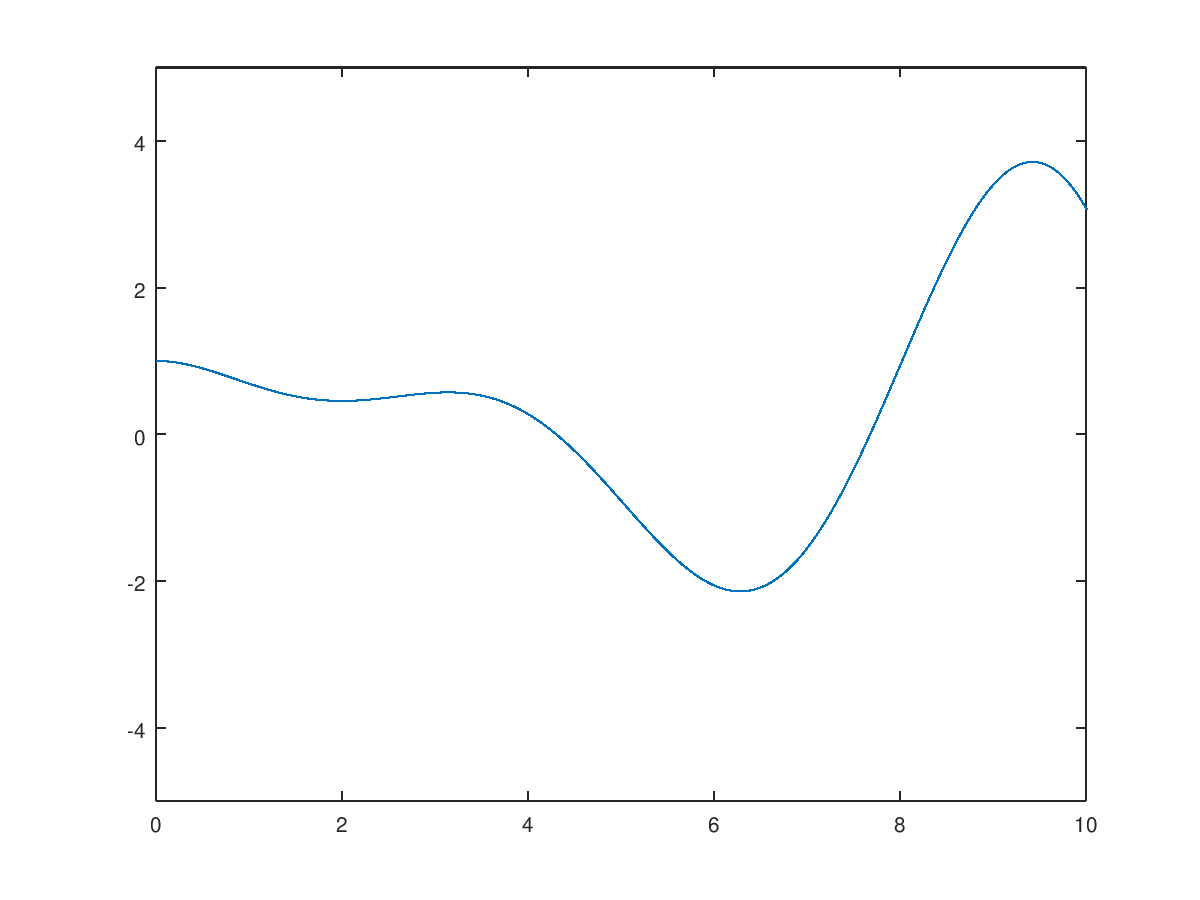
\includegraphics[scale=0.5]{hw0_p1_1}
\caption{$x(t)$ vs. $t$}
\label{fig:universe}
\end{figure}
\begin{figure}[h!]
\centering
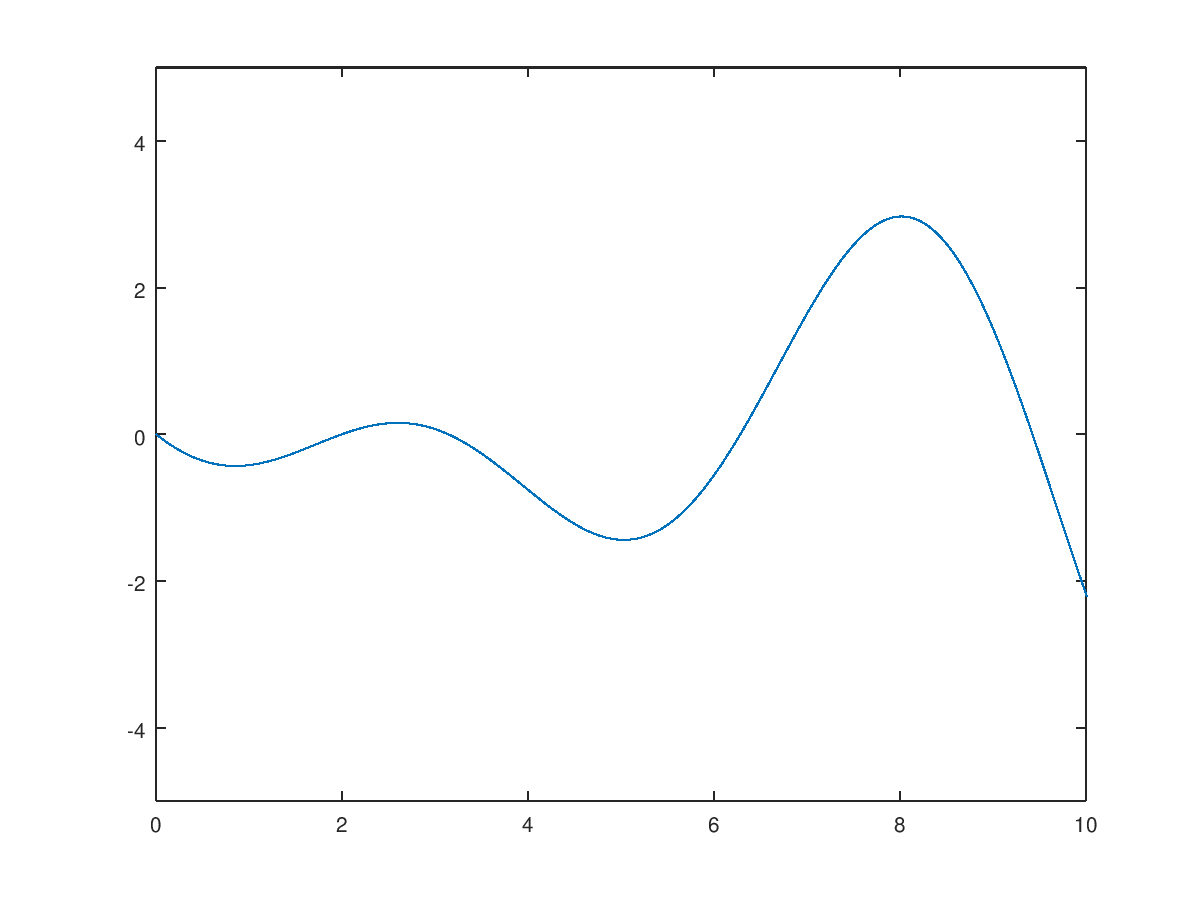
\includegraphics[scale=0.5]{hw0_p1_2}
\caption{$\dot x (t)$ vs. $t$}
\label{fig:universe}
\end{figure}
%oh jeez I really fucking hate latex
\begin{verbatim}












\end{verbatim}
\section{Problem 2}


\emph{Problem Statement}

Find the fourier series for a square wave with amplitude 0.5 and period 1.
\emph{Soution}

We can set up the solution for the fourier series as follows:

\[
   b_n = \frac{1}{L}(\int_{0}^{L} \sin{\left (\frac{\pi n t}{L} \right )}\, dt 
   +\int_{-L}^{0} \left(- \sin{\left (\frac{\pi n t}{L} \right )}\right)\, dt)
   = - \frac{2  \cos{\left ( \pi n \right )}}{\pi n} + \frac{2 }{\pi n}
\]
Therefore if L = 1/2:
\[
b_n =
\begin{cases}
\frac{4}{\pi n}, &  n = 1,3,5... \\
0, & n= 2,4,6...\\
\end{cases}
\]
Since the function is odd we know that:
\[ 
a_n = 0 
\]
Since the average value of the function is 0 we know that:
\[
a_0 = 0
\]

\begin{verbatim}
\end{verbatim}

\section{Problem 3}

Solving for eigenvalues of the matrix $A$ 
\[
A = \begin{bmatrix}0&1\\[0.3em]
-3&2\\[0.3em]
\end{bmatrix}
\]
\[
det \begin{bmatrix}0 - \lambda&1\\[0.3em]
-3&2-\lambda\\[0.3em]
\end{bmatrix}
= (0 - \lambda)(2 - \lambda) - (1)(-3) = -\lambda*(-\lambda + 2) + 3 = 0
\]

The eigenvalues are the values of $\lambda$ such that the determinant equals zero, therefore:
\[
\lambda = \left [ 1 - \sqrt{2} i, \quad 1 + \sqrt{2} i\right ]
\]

These answers were then confirmed with matlabs eig function. The output is shown below:

\begin{verbatim}
>> A = [0 1;-3 2]
A =

   0   1
  -3   2

>> eig(A)
ans =

   1.0000 + 1.4142i
   1.0000 - 1.4142i

\end{verbatim}


\section{Problem 4}
To solve for the pendulum system we will find the torque on the pendulum in polar coordinates. The torque from gravity is written as:
\[
\tau _g = - g l m \sin{\left (\theta \right )}\]
The torque from the spring is written as:

\[
\tau_s = - \frac{4 k l^{2} \sin{\left (\theta \right )} \cos{\left (\theta \right )}}{9}
\]
The torque from friction is written as:
\[
\tau_f = -b \dot \theta
\]
For small angles we can make the approximations that:
\[
sin(\theta) = \theta
\]

\[
cos(\theta) = 1
\]
And linearize the equation as such:
\[
ml^2 \ddot \theta  = -b \dot \theta - \theta g l m- \frac{4 \theta k l^{2}}{9}\]
Assuming the solution takes the form:
\[
\theta (t) = e^{rt}
\]
We can solve for r:
\[
b r + g l m + \frac{4 k l^{2}}{9} + l^{2} m r^{2} = 0\]

\[
r =
\left [ \frac{- 3 b + \sqrt{9 b^{2} - 36 g l^{3} m^{2} - 16 k l^{4} m}}{6 l^{2} m}, \quad - \frac{3 b + \sqrt{9 b^{2} - 36 g l^{3} m^{2} - 16 k l^{4} m}}{6 l^{2} m}\right ]\]

%\bibliographystyle{plain}
\bibliography{references}
\end{document}
